% Important: If latex complains about unicode characters,
% please use "\usepackage[utf8x]{inputenc}" in your preamble
% You can change the size of the picture by putting it into the construct:
% 1) \resizebox{10cm}{!}{"below picture"} to scale horizontally to 10 cm
% 2) \resizebox{!}{15cm}{"below picture"} to scale vertically to 15 cm
% 3) \resizebox{10cm}{15cm}{"below picture"} a combination of above two
% It is not recomended to use the scale option of the tikzpicture environment.
\resizebox{4.5cm}{!}{
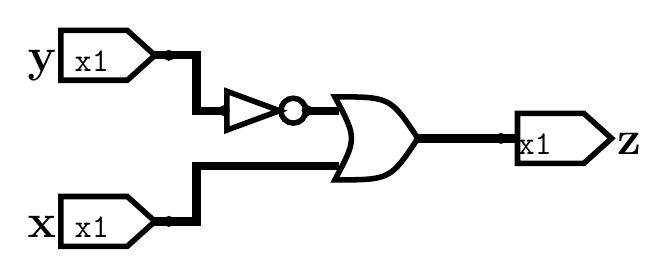
\begin{tikzpicture}[x=1pt,y=-1pt,line cap=rect]
\def\logisimfontA#1{\fontfamily{cmr}{#1}} % Replaced by logisim, original font was "SansSerif"
\def\logisimfontB#1{\fontfamily{cmtt}{#1}} % Replaced by logisim, original font was "Monospaced"
\definecolor{custcol_0_0_0}{RGB}{0, 0, 0}
\definecolor{custcol_ff_ff_ff}{RGB}{255, 255, 255}
\draw [line width=3.0pt, custcol_0_0_0 ]  (146.0,45.0) -- (176.0,45.0) ;
\draw [line width=3.0pt, custcol_0_0_0 ]  (106.0,35.0) -- (116.0,35.0) -- (116.0,35.0) ;
\draw [line width=2.0pt, custcol_0_0_0 ]  (146.0,45.0) .. controls  (136.0,30.0)  ..  (116.0,30.0) .. controls  (124.0,45.0)  ..  (116.0,60.0) .. controls  (136.0,60.0)  ..  (146.0,45.0) -- cycle ;
\draw [line width=2.0pt, custcol_0_0_0 ]  (96.0,35.0) -- (77.0,28.0) -- (77.0,42.0) -- cycle;
\draw [line width=2.0pt, custcol_0_0_0]  (101.0,35.0) ellipse (4.5 and 4.5 );
\fill [line width=2.0pt, custcol_0_0_0]  (106.0,35.0) ellipse (2.0 and 2.0 );
\fill [line width=2.0pt, custcol_0_0_0]  (76.0,35.0) ellipse (2.0 and 2.0 );
\draw [line width=3.0pt, custcol_0_0_0 ]  (180.0,45.0) -- (177.0,45.0) ;
\draw [line width=2.0pt, custcol_0_0_0 ]  (206.0,36.0) -- (216.0,45.0) -- (206.0,54.0) -- (182.0,54.0) -- (182.0,36.0) -- cycle;
\logisimfontB{\fontsize{12pt}{12pt}\selectfont\node[inner sep=0, outer sep=0, custcol_0_0_0, anchor=base west] at  (182.0,51.0)  {x1};}
\logisimfontA{\fontsize{16pt}{16pt}\fontseries{bx}\selectfont\node[inner sep=0, outer sep=0, custcol_0_0_0, anchor=base west] at  (218.0,51.0)  {z};}
\fill [line width=2.0pt, custcol_0_0_0]  (176.0,45.0) ellipse (2.0 and 2.0 );
\draw [line width=3.0pt, custcol_0_0_0 ]  (51.0,75.0) -- (56.0,75.0) -- (66.0,75.0) -- (66.0,55.0) -- (116.0,55.0) -- (116.0,55.0) ;
\draw [line width=2.0pt, custcol_0_0_0 ]  (41.0,84.0) -- (51.0,75.0) -- (41.0,66.0) -- (17.0,66.0) -- (17.0,84.0) -- cycle;
\logisimfontB{\fontsize{12pt}{12pt}\selectfont\node[inner sep=0, outer sep=0, custcol_0_0_0, anchor=base west] at  (22.0,81.0)  {x1};}
\logisimfontA{\fontsize{16pt}{16pt}\fontseries{bx}\selectfont\node[inner sep=0, outer sep=0, custcol_0_0_0, anchor=base west] at  (5.0,81.0)  {x};}
\fill [line width=2.0pt, custcol_0_0_0]  (56.0,75.0) ellipse (2.0 and 2.0 );
\draw [line width=3.0pt, custcol_0_0_0 ]  (51.0,15.0) -- (56.0,15.0) -- (66.0,15.0) -- (66.0,35.0) -- (76.0,35.0) ;
\draw [line width=2.0pt, custcol_0_0_0 ]  (41.0,24.0) -- (51.0,15.0) -- (41.0,6.0) -- (17.0,6.0) -- (17.0,24.0) -- cycle;
\logisimfontB{\fontsize{12pt}{12pt}\selectfont\node[inner sep=0, outer sep=0, custcol_0_0_0, anchor=base west] at  (22.0,21.0)  {x1};}
\logisimfontA{\fontsize{16pt}{16pt}\fontseries{bx}\selectfont\node[inner sep=0, outer sep=0, custcol_0_0_0, anchor=base west] at  (5.0,21.0)  {y};}
\fill [line width=2.0pt, custcol_0_0_0]  (56.0,15.0) ellipse (2.0 and 2.0 );
\end{tikzpicture}
}
